\chapter{Evoluzione}
\thispagestyle{empty}
Il compito di un sistema operativo è fornire ai programmi utente un'interfaccia semplificata con l'hardware.
La maggior parte dei sistemi operativi reali sono scritti in linguaggio C.

\begin{figure}[h!]
    \centering
    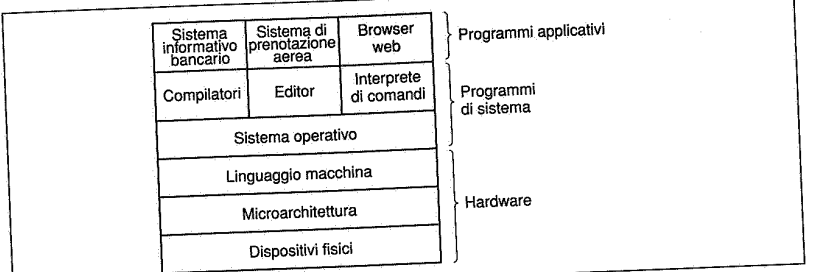
\includegraphics[width=0.7\linewidth]{assets/calcolatore1.png}
    \caption{Struttura di un generico calcolatore}
\end{figure}

I dispositivi di ingresso/uscita sono controllati mediante il caricamento di valori in speciali \textbf{registri di dispositivo}: per esempio, è possibile ordinare ad un disco di eseguire una lettura caricando nei suoi registri di dispositivo il valore dell'indirizzo su disco, l'indirizzo in memoria principale, numero di byte e direzione (lettura o scrittura).

Il sistema operativo nasconde parzialmente l'hardware e dà al programmatore un insieme di istruzioni più pratico con cui lavorare.

Esso è (normalmente) quella porzione di software che viene eseguita in modalità kernel, i compilatori e gli editor vengono eseguiti in modalità utente.
In qualche sistema è difficile tracciare un confine netto: tutto ciò che vie-
ne eseguito in modalità kernel fa ovviamente parte del sistema operativo, ma e possibile che alcuni programmi che non vengono eseguiti in questa modalità siano parte di esso o, almeno, gli siano strettamente collegati.

Il sistema operativo è normalmente protetto con meccanismi hardware da ogni tentativo di modifica da parte dell'utente.

\section{Cos'è un sistema operativo}
Il sistema operativo realizza due funzionalita che sono praticamente scorrelate, \textit{estende la macchina} e \textit{gestisce risorse}.

Per quanto riguarda la prima funzionalità: il sistema operativo fornisce una varietà di servizi, di cui i programmi possono usufruire attraverso istruzioni speciali dette chiamate di sistema (\textbf{system call}).

E per la seconda: tiene traccia di chi stia usando quale risorsa, soddisfa le richieste delle risorse, contabilizza l'uso e media richieste conflittuali provenienti da programmi e utenti diversi.
La gestione delle risorse comporta la loro condivisione sotto due aspetti: rispetto al tempo e rispetto allo spazio. Con quest'ultimo si intende per esempio la condivisione della memoria principale: essa è normalmente
ripartita fra diversi programmi in esecuzione, così che possano stare in memoria contemporaneamente (per esempio, allo scopo di fare a turno per l'uso della CPU).

\section{Storia dei sistemi operativi}

\subsection{La prima generazione}
Meta degli anni '40.
Macchine enormi, riempivano intere stanze ed erano composte da centinaia di migliaia di \textbf{valvole}.

Tutta la programmazione era effettuata in \textbf{linguaggio macchina} e non vi era traccia di alcun sistema operativo.

All'inizio degli anni '50 iniziarono ad essere introdotte le \textbf{schede perforate}. Ora era possibile scrivere i programmi su di esse e leggerli tramite il calcolatore invece di usare gli spinotti.

\subsection{La seconda generazione}
Innovazione: \textbf{transistor}.

Il costo dei calcolatori, di molti milioni di dollari, poteva essere affrontato solo da grosse compagnie, dalle agenzie governative o dalle università. Per far girare un \textbf{job} (cioè un programma o un insieme di programmi), un programmatore doveva prima scrivere il
programma su carta (in FORTRAN\footnote{\textit{FOR}mule \textit{TRAN}slator} o in assembler), poi doveva copiarlo su schede perforate, infine doveva portare il pacchetto delle schede nella stanza dove venivano raccolti i programmi e darlo ad uno degli operatori. Dopodiché poteva andare a prendersi un caffè in attesa dei risultati in uscita. Appena il calcolatore aveva terminato il job in esecuzione in quel momento, qualsiasi cosa fosse, un operatore andava alla stampante, prelevava quanto prodotto in uscita dal job e lo portava nella stanza dove venivano distribuiti i risultati delle elaborazioni, in modo che il programmatore lo potesse ritirare più tardi; quindi prendeva uno dei pacchetti di schede dalla stanza di raccolta dei programmi e lo faceva leggere al calcolatore.  Se risultava necessario anche il compilatore FORTRAN, l'operatore lo doveva prendere dall'archivio e farlo leggere al calcolatore. Gran parte del tempo di elaborazione andava quindi sprecato mentre gli operatori andavano avanti e indietro per la sala macchine.

Per ridurre il tempo la soluzione che venne adottata nella maggior parte dei casi fu quella dei \textbf{sistemi batch} (sistemi di elaborazione a lotti). L'idea era quella di raccogliere un intero cassetto di job nella stanza dedicata alla raccolta dei programmi e di farli trasferire su nastro magnetico da un piccolo calcolatore (relativamente) poco costoso,
Dopo circa un'ora durante la quale veniva raccolto un batch (lotto) di lavori, il nastro veniva riavvolto e portato nella sala macchine, dove veniva montato sul lettore di nastri. L'operatore caricava quindi un programma speciale (l'antenato degli attuali sistemi operativi) che leggeva il primo job e lo eseguiva; i dati in uscita, anziché venire stampati, venivano registrati su un secondo nastro magnetico. Dopo la fine di ognuno dei job, il sistema operativo leggeva in maniera automatica il prossimo job dal nastro di ingresso e lo mandava in esecuzione. Quando l'intero lotto di lavori era stato eseguito, l'operatore rimuoveva i nastri di ingresso e di uscita, li sostituiva con quelli di un nuovo lotto di lavori e prendeva il nastro di uscita per stamparne i dati fuori linea, cioè senza essere direttamente collegato al calcolatore principale.

\begin{figure}[h!]
    \centering
    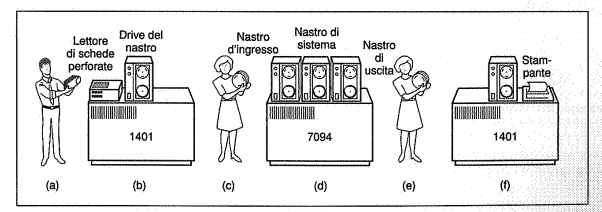
\includegraphics[width=0.7\linewidth]{assets/batch1.png}
    \caption{Uno dei primi sistemi di elaborazione batch}
\end{figure}

\begin{figure}[h!]
    \centering
    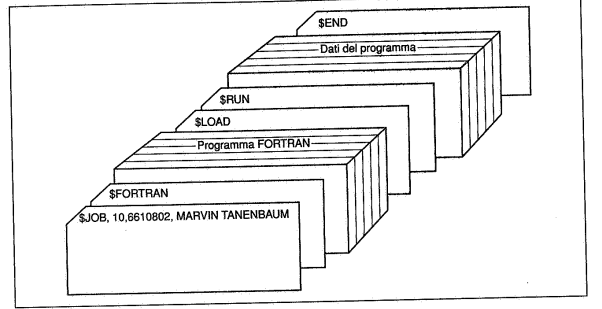
\includegraphics[width=0.7\linewidth]{assets/job1.png}
    \caption{Struttura di un tipico job FMS}
\end{figure}

\subsection{La terza generazione}
Innovazione: \textbf{circuiti integrati}.

I sistemi di terza generazione resero popolare la tecnica della \textbf{multiprogrammazione}: essa consisteva nel dividere la memoria centrale in alcune partizioni, con un job diverso per ogni partizione; mentre un job rimaneva in attesa del completamento di una certa attività di ingresso/uscita, la CPU poteva essere usata da un altro job e quando si riusciva a tenere in memoria un numero sufficiente di job contemporaneamente, si riusciva a mantenere occupata la CPU quasi per il 100 per cento del tempo.

\begin{figure}[h!]
    \centering
    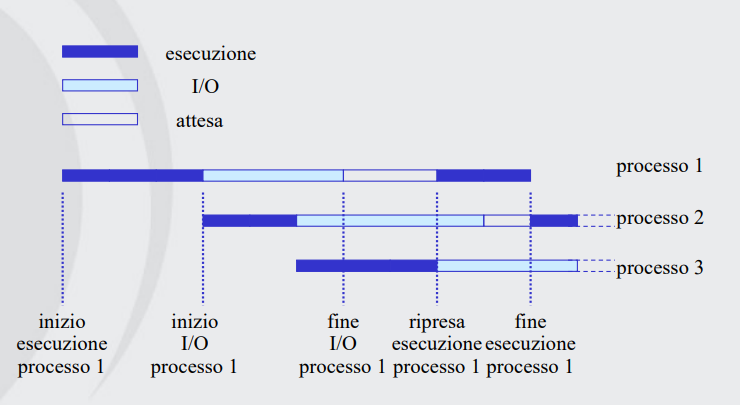
\includegraphics[width=0.7\linewidth]{assets/multiprogrammazione1.png}
    \caption{Esempio di multitasking}
\end{figure}

Un'altra caratteristica importante dei sistemi operativi della terza generazione era quella di permettere la lettura dei job dalle schede al disco non appena le schede venivano portate alla sala macchine. Poi, non appena il job in esecuzione terminava, il sistema operativo poteva caricare un nuovo job dal disco nella partizione di memoria che si era resa disponibile e mandarlo in esecuzione. Questa tecnica viene chiamata \textbf{spooling}.

Il desiderio di un tempo di risposta veloce preparò la strada al \textbf{timesharing} (condivisione di tempo), una variante della multiprogrammazione nella quale ogni utente aveva a disposizione un terminale in linea. Nei sistemi timesharing, se 20 utenti erano collegati contemporaneamente e 17 di loro stavano pensando, bevendo caffè o parlando, la CPU poteva essere assegnata all'esecuzione a turno dei tre job che in quel momento richiedevano il servizio.

\begin{figure}[h!]
    \centering
    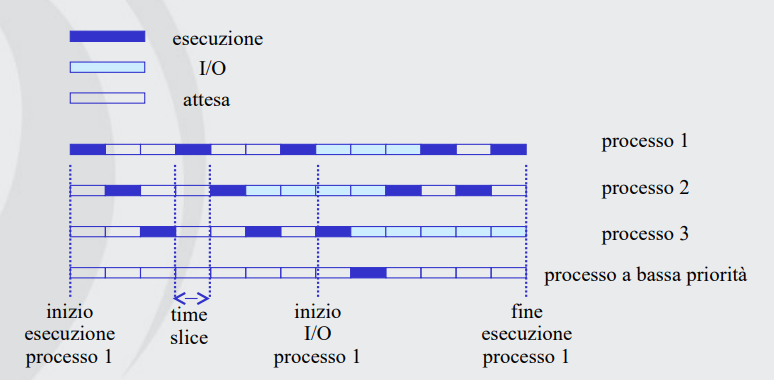
\includegraphics[width=0.7\linewidth]{assets/timesharing1.png}
    \caption{Esempio di condivisione del tempo}
\end{figure}

\subsection{La quarta generazione}

Innovazione: \textbf{VLSI} (Very Large Scale Integration).

Nasce l'era dei personal computer. MS-DOS domina il mercato.

Negli anni '60 viene introdotta per la prima volta la \textbf{GUI}, completa di finestre, icone, menù e mouse.

Negli anni '80 iniziano ad essere utilizzati i \textbf{sistemi operativi di rete} e i \textbf{sistemi operativi distribuiti}.

Nei primi gli utenti sono a conoscenza dell'elevato numero di calcolatori e possono accedere alle macchine remote; ogni macchina ha il proprio sistema operativo e i propri utenti.

Nei secondi invece, il sistema distribuito appare agli utenti come un singolo sistema monoprocessore. Essi non sanno dove i propri file sono allocati e non sanno dove i loro programmi vengono fatti girare.

\subsection{La quinta generazione}
Sono i sistemi operativi mobile.

Tra la grande varietà di sistemi operativi presenti sul mercato attuale si vuole dare una spiccata importanza ai sistemi operativi \textbf{real-time}.
Quando deve essere eseguita un azione \textit{assolutamente} in un dato momento o intervallo di tempo si parla di sistemi real-time.
Una categoria esemplificativa sono i sistemi digitali audio o quelli multimediali, essi fanno parte della categoria \textit{soft real-time systems}.


\section{L'hardware dei calcolatori}
I componenti principali che compongono un calcolatore sono:
\begin{itemize}
    \item Processore
    \item Memoria
    \item Dispositivi in/out
    \item Bus
\end{itemize}

\subsection{Processore}
Il processore è un chip che contiene una o più CPU.
Il "cervello" di un calcolatore è la CPU, che recupera le istruzioni dalla memoria e le esegue. 
Essa piò essere composta da più \textit{core}, che sono l'unità di elaborazione base di una CPU.

\begin{figure}[h!]
  \begin{subfigure}{.5\textwidth}
  \centering
    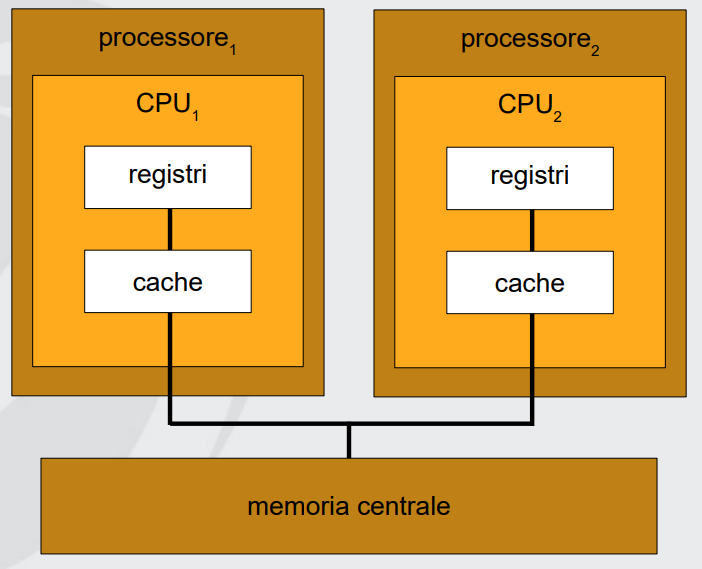
\includegraphics[width=0.7\linewidth]{assets/multiprocessore1.png}
    \caption{multiprocessore}
  \end{subfigure}%
  \begin{subfigure}{.5\textwidth}
  \centering
    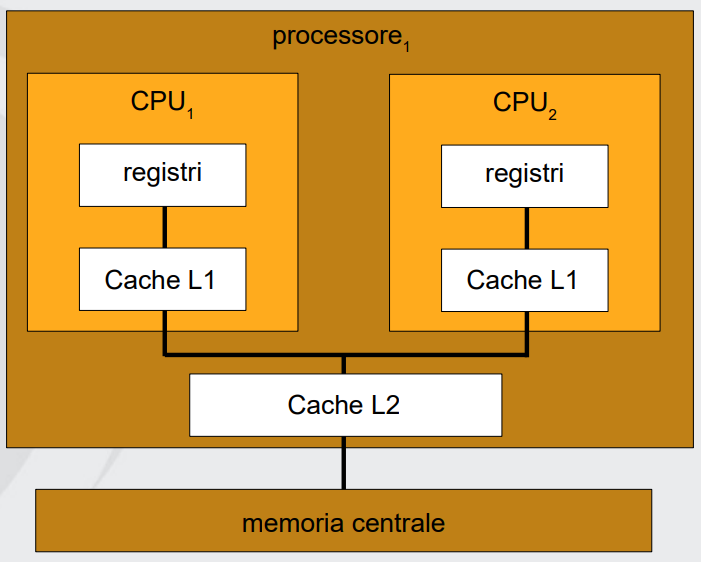
\includegraphics[width=0.7\linewidth]{assets/multicore1.png}
    \caption{multicore}
  \end{subfigure}
  \caption{Architetture con multieleborazione}
\end{figure}

Occorre fare attenzione poiché aggiungere nuove CPU aumenta le prestazioni relative al calcolo ma peggiora quelle relative all'accesso alla memoria. Una possibile soluzione tuttavia può essere fornire a ciascuna CPU una propria memoria locale accessibile da un piccolo bus. I sistemi che implementano questa soluzione sono detti sistemi \textbf{NUMA}: ovvero ad accesso non uniforme alla memoria. La pecca più grande è lo spreco di tempo in quei casi in cui una CPU deve accedere alla memoria di un'altra.

\begin{figure}[!ht]
    \centering
    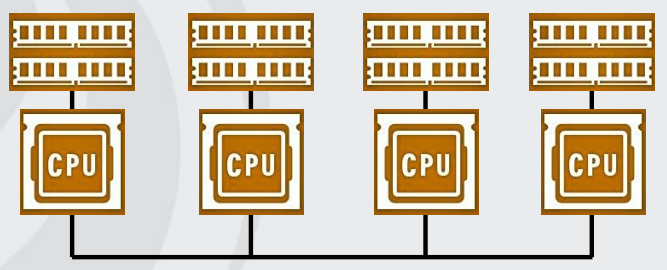
\includegraphics[width=0.7\linewidth]{assets/numa1.png}
    \caption{sistema NUMA}
\end{figure}

Il ciclo di azioni base eseguito da ogni CPU consiste nel recuperare la prima istruzione dalla memoria, decodificarla per determinarne tipo e operandi, ed eseguirla e quindi recuperare, decodificare, eseguire le istruzioni seguenti. In questo modo vengono completati i programmi. Ogni CPU è in grado di eseguire un insieme di istruzioni specifico.

Tutte le CPU contengono, al loro interno, alcuni registri per mantenervi variabili chiave e risultati temporanei. Normalmente, l'insieme di istruzioni ne contiene quindi alcune per caricare una parola dalla memoria in un registro e per depositare una parola da un registro alla memoria.

La maggior parte dei calcolatori ha parecchi registri speciali disponibili al programmatore. Uno di questi è il \textit{program counter}, o contatore di programma, che contiene l'indirizzo di memoria della prossima istruzione da andare a prendere (\textit{fetch}); dopo che l'istruzione è stata recuperata, il program counter viene aggiornato per puntare all'istruzione successiva. 
Un altro registro è lo \textit{stack pointer} o puntatore alla pila, che punta alla cima dello stack corrente in memoria; tale stack o pila contiene una struttura (frame) per ogni procedura che è stata iniziata ma non è ancora terminata, ognuna delle quali contiene i parametri d'ingresso, e le variabili locali e temporanee che non vengono mantenuti nei registri.

Le CPU moderne hanno unità separate per le tre fasi di recupero, decodifica e esecuzione, così che, mentre è in esecuzione l'istruzione n, potrebbero essere in grado di decodificare l'istruzione n+1 e recuperare l'istruzione n+2. Un'organizzazione di questo tipo è detta \textit{pipeline}.

La maggior parte delle CPU hanno due modalità, quella kernel e quella utente.
Il sistema operativo viene eseguito nella prima modalità mentre i programmi utente nella seconda. Per ottenere servizi dal sistema operativo, un programma deve eseguire una chiamata di sistema o system call, che esegue una trap al kernel e invoca il sistema operativo: l'istruzione TRAP cambia da modalità utente a modalità kernel e avvia il sistema operativo.
Gli elaboratori hanno altre istruzioni di tipo trap oltre a quella per eseguire chiamate di sistema: la maggior parte delle trap sono causate dall'hardware per avvisare di una situazione eccezionale, come può essere un tentativo di divisione per 0 o un underflow nell'aritmetica a virgola mobile. In ogni caso, il sistema operativo ottiene il controllo, e deve decidere cosa fare.

\subsection{Memoria (facoltativo)}
La memoria ideale dovrebbe essere estremamente veloce (più veloce dell'esecuzione di un'istruzione, in modo che la CPU non sia rallentata).
Essa è costruita come una gerarchia di strati.

\begin{wrapfigure}{l}{0.4\textwidth}
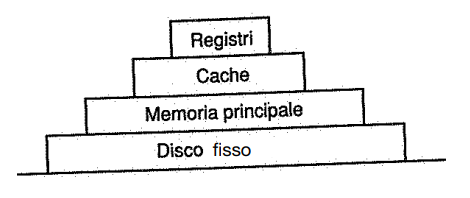
\includegraphics[width=1\linewidth]{assets/memoria1.png} 
\caption{Tipica gerarchia di una memoria}
\end{wrapfigure}

\phantom{ }
\begin{itemize}
    \item i \textit{registri}: interni alla CPU.
    \item la \textit{cache}: controllata dall'hardware.
    \item la \textit{memoria principale}: anche chiamata \textbf{RAM} (Random Access Memory).
    \item \textit{hard disk}.
\end{itemize}

In aggiunta ai tipi di memoria discussi sopra, molti elaboratori hanno una piccola porzione di memoria ad accesso casuale non volatile; a differenza della RAM, la memoria non volatile non perde il suo contenuto nel momento in cui viene tolta la corrente. La \textbf{ROM} (Read Only Memory) è programmata in fabbrica e non può essere modificata in seguito. Su qualche elaboratore, il programma di avvio (bootstrap loader) usato per avviare l'elaboratore stesso è contenuto in ROM.

Anche le EEPROM (Electrically Erasable ROM, ROM cancellabili elettricamente) e le flash RAM non sono volatili, ma al contrario delle ROM possono essere cancellate e riscritte. Tuttavia, per scrivere su di esse occorrono tempi di qualche ordine di grandezza più lunghi di quelli per scrivere sulle RAM,

Un altro tipo di memoria è la memoria CMOS, che è volatile ed è utilizzata da molti elaboratori per memorizzare ora e data corrente.
La memoria CMOS è utilizzata perché consuma così poca corrente che la batteria originale installata in fabbrica dura spesso diversi anni. Tuttavia, quando inizia a scaricarsi, può sembrare che l'elaboratore abbia il morbo di Alzheimer, dimenticandosi cose che ha saputo per anni, come il disco dal quale eseguire il boot.

Per tenere due o più programmi in memoria principale occorre risolvere due problemi: 
\begin{enumerate}
    \item gestire la rilocazione.
    \item proteggere i programmi l'uno dall'altro e il kernel dai programmi.
\end{enumerate}
%
Il primo si risolve nella conversione dell'indirizzo generato dal programma, chiamato indirizzo virtuale, nell'indirizzo utilizzato dalla memoria, chiamato indirizzo fisico. Il dispositivo che effettua il controllo e la corrispondenza è detto MMU (Memory Management Unit).
%
Per il secondo si usa una coppia di registri speciali, il \textit{registro base} e il \textit{registro limite}. Quando un programma viene eseguito, il registro base è impostato al punto di inizio del suo codice,e il registro limite contiene il totale dello spazio occupato dal codice e dai dati del programma. Quando un'istruzione deve essere recuperata, l'hardware controlla che il program counter sia minore del registro limite e, se è così, lo somma al contenuto del registro base e spedisce il risultato alla memoria.Il registro base rende impossibile che il programma si riferisca a parti di memoria al di sotto di se stesso, e il registro limite rende impossibile che si riferisca a parti di memoria superiori al programma stesso.

Il passare da un programma ad un altro è generalmente una operazione costosa, essa è denominata \textit{cambio di contesto}.

\subsection{I dispositivi input/output (facoltativo)}

I dispositivi di ingresso/uscita generalmente sono composti da due parti: un controllore ed il dispositivo stesso.

Il controllore è un chip posto su una scheda estraibile, che controlla fisicamente il dispositivo, ed accetta comandi dal sistema operativo. Il suo compito è quello di presentare un interfaccia semplificata al sistema operativo. I controllori spesso contengono piccoli elaboratori embedded.

Dato che ogni tipo di controllore è diverso, sono necessari software diversi per controllare ognuno di essi; il software che parla al controllore, che da i comandi e accetta le risposte, è detto device \textit{driver}. Ogni fabbricante di controllori deve fornire un driver per ogni sistema operativo che supporta. Per essere usato, un driver deve essere posto nel sistema operativo per essere eseguito in modalità kernel: occorre quindi un riavvio ogni volta che va installato un nuovo driver (tranne in particolari casi come per gli \textit{hot pluggable device}, in quel caso si fa in modo che non sia necessario). Ogni controllore ha un piccolo numero di registri che vengono usati per comunicare con esso. Per esempio, un controllore di disco minimale potrebbe avere registri che specificano l'indirizzo su disco, l'indirizzo di memoria, il numero di settori e la direzione (lettura o scrittura); per attivare il controllore, il driver riceve un comando dal sistema operativo, quindi lo traduce nei valori appropriati da scrivere nei registri del dispositivo.
Su qualche elaboratore, i registri di dispositivo sono messi in corrispondenza con indirizzi all'interno dello spazio di indirizzamento del sistema operativo.

Ci sono tre modi per eseguire operazioni di ingresso/uscita:
\begin{enumerate}
    \item Polling.
    \item Interrupt.
    \item Accesso diretto alla memoria (\textit{DMA}).
\end{enumerate}

\subsection{I bus (facoltativo)}

 L'USB (Universal Serial Bus) è stato inventato per permettere di collegare al calcolatore tutti i dispositivi di ingresso/uscita lenti, come la tastiera e il mouse. Utilizza un piccolo connettore a quattro fili, due dei quali forniscono energia elettrica ai dispositivi USB. Tutti i dispositivi USB condividono un solo driver di dispositivo USB.

 Il brutto arrivava quando l'utente comprava una scheda sonora e un modem e capitava che entrambi usassero, diciamo, l'interruzione 4. Per ovviare al problema si utilizza il \textit{plug and play}, esso permette al sistema di raccogliere automaticamente le informazioni relative ai dispositivi di ingresso/uscita, assegnare in modo centralizzato i livelli di interruzione e gli indirizzi di ingresso/uscita, e comunicare ad ogni scheda il proprio numero. 
 
 Sulla scheda madre risiede un programma detto \textit{BIOS} (Basic Input Output System), che contiene software di basso livello per l'ingresso/uscita, comprese le procedure per leggere la tastiera, scrivere sul video e fare ingresso/uscita su disco. Oggigiorno, è contenuto in una flash RAM, che è non volatile e può essere aggiornata dal sistema operativo quando vengono rilevati dei bachi nel BIOS. Il BIOS determina il dispositivo di memoria da cui effettuare l'inizializzazione (boot) provando i dispositivi elencati in una lista memorizzata nella memoria CMOS, che l'utente può modificare eseguendo il configuratore del BIOS immediatamente dopo aver acceso il calcolatore.



